\section{T�cnica}

\outline{Descrever o processo de c�lculo do tempo de acesso ao meio, e onde foi baseado.}


Em qualquer t�cnica de sincroniza��o de rel�gios em sistemas distribu�dos, os n�s tem que dizer um ao outro o seu tempo local. A Figura \ref{fig:diagrama} ilustra esse cen�rio. O n� emissor armazena o seu tempo local ${t_1}'$ na mensagem de sincroniza��o no tempo $t_1$ e ordena o envio da mensagem. Devido as incertezas aleat�rias do acesso ao meio, o emissor s� recebe o acesso ao meio no tempo $t_2$ e come�a a enviar a mensagem. O \textit{tempo de acesso ao meio} � definido por $t_2 - t_1$. A mensagem propaga-se sobre o meio por um intervalo de tempo $tp$ at� que atinge o r�dio do receptor no tempo $t_3$. O \textit{tempo de propaga��o} � definido por $tp$. Devido as pol�ticas de manipula��o de interrup��o e processamento do cabe�alho do pacote, o n� receptor marca o \textit{timestamp} do recebimento no tempo $t_4$ com o seu tempo local ${t_4}''$. O \textit{tempo de processamento} � dado por $t_4 - t_3$.



\begin{figure}[htbp]
	\centering
		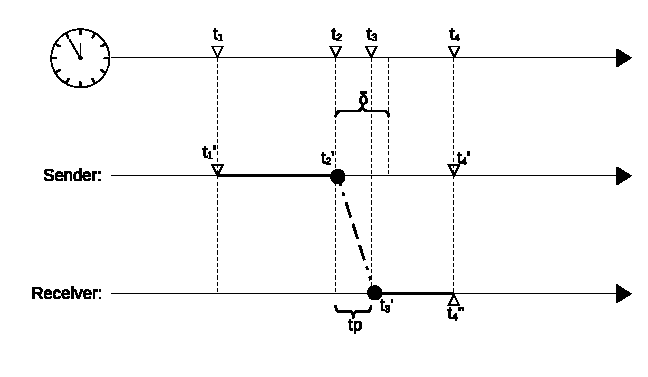
\includegraphics[width=\linewidth]{figuras/diagrama.eps}
	\caption{Syncronization steps.}
	\label{fig:diagrama}
\end{figure}


A imprecis�o de sincroniza��o acontece porque o n� de receptor pensa que no tempo $t_4$ o emissor tem o tempo ${t_1}'$ e o receptor tem o tempo ${t_4}''$. Como podemos ver na Figura \ref{fig:diagrama}, isso n�o � verdade. No tempo $t_4$, o n� emissor tem o tempo ${t_4}' = {t_1}' + \mbox{\textit{tempo de acesso ao meio}} + \mbox{\textit{tempo de propaga��o}} + \mbox{\textit{tempo processamento}}$. O \textit{timestamp} na camada MAC faz \textit{tempo de acesso ao meio} e \textit{tempo de processamento} igual a zero. Desde que o \textit{tempo de propaga��o} � desprez�vel ($\sim 1\mu{s}$) \cite{maroti2004}, algumas pol�ticas de sincroniza��o -- incluindo o FTSP -- podem atingir uma precis�o muito boa. Contudo, sem o \textit{timestamp} na camada MAC, esses tempo n�o s�o negligenci�veis e tem que ser calculados. 
